\section{Results and discussion} \label{Results-and-discussion}

We employed the SERPENT-2 Monte Carlo code to calculate all parameters herein.
We used the ENDF/B-VII.0 \cite{CHADWICK20062931} cross section library for all calculations in the current work. The statistical error in $k_{eff}$ is $\leq$ $25$ $pcm$.
The initial calculation state of a full 3D model of the SD-TMSR is identified by normal operation 
conditions (see Table~\ref{tab:table1}) and fully withdrawn control rod 
clusters. 
The obtained results including excess reactivity, control rod 
worth, shutdown margin, interference effects (shadowing effects), etc. are discussed below.

\subsection{Excess reactivity}

The excess reactivity $\rho$$_e$ is calculated by using equation~\ref{Equ:1} at zero burnup (steady-state 
calculation), when all control rods are fully withdrawn. The $\rho_e$ for $^{233}$U, 
reactor-grade Pu, and TRU used as initial fissile material are listed in Table~\ref{tab:excess}.
For $^{233}$U case \cite{ashraf2020Strategies} the initial excess reactivity is about $1180\pm28$ $pcm$, however, the maximum observed excess reactivity is $1344\pm25$ $pcm$ during 60 effective full-power years (EFPY) of operation (see Figure~\ref{fig:keff_25} after $\approx$ 8 EFPY of operation). TRU has a great amount of thermal neutron absorbers, therefore, the SD-TMSR becomes subcritical relatively quickly. Previous studies showed that for promising fueling scenarios (e.g., TRU/$^{232}$Th), large excess reactivity is required for long-term core operation \cite{ashraf2020Strategies,betzler2017assessment,rykhlevskii_fuel_2019}. The proposed reactivity control system must compensate such reactivity at startup and during burnup.

\begin{table}  %[!hb]
	\caption{The excess reactivity at startup for the SD-TMSR core with different initial fissile materials.}
	\vspace{0.1in}
	\begin{tabularx}{\textwidth}{p{3cm} s s s}
		\hline
		Initial fissile materials       				&  $^{233}$U & reactor-grade Pu&  TRU \\
		\hline
		$\rho_e$					& $1180\pm28$ $pcm$ & $2330\pm30$ $pcm$ & $4800\pm35$ $pcm$ \\
		\hline
	\end{tabularx}
	\label{tab:excess}
\end{table}

\begin{figure}
	\centering
	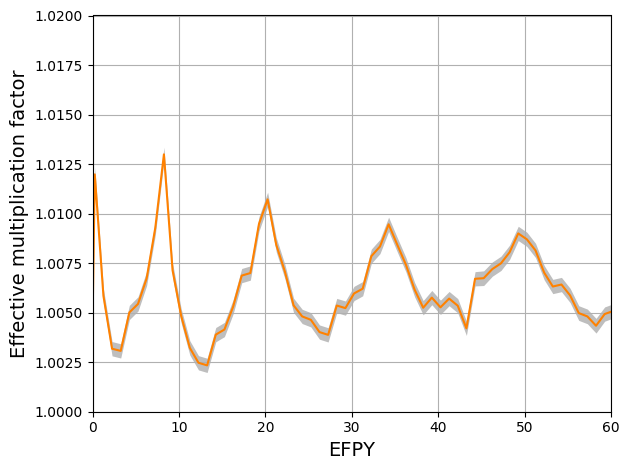
\includegraphics[width=\textwidth]{keff_25.png}
	\vspace{-0.5in}
	\caption{Uncontrolled effective multiplication factor during 60 EFPY of reactor operation
		including periodic $^{233}$U/$^{232}$Th insertion (confidence interval $\pm\sigma$ is shaded) \cite{ashraf2020whole}.} 
	\label{fig:keff_25}
\end{figure}

\subsection{Control rod parameters}

The control rod parameters including control rod worth (CRW), interference 
between CR clusters, and integral and differential control rod worths are 
described in this work. Table~\ref{tab:worth} shows calculated CRW and the amplification 
factor (A$_{CRi}$) for six different 
absorbers. The types of interference for all different 
absorbers are listed in Table ~\ref{tab:table25}. Fuel salt composition of LiF-BeF$_2$-ThF$_4$-$^{233}$UF$_4$ at 70-17.5-12.3-0.2 mole\% is used to generate the results listed in Tables~\ref{tab:worth} and ~\ref{tab:table25}. However, Table~\ref{tab:table51} summarizes the CRW of all CRs, CSD, and SSD for SD-TMSR initially loaded by reactor-grade Pu and TRU. 

\begin{sidewaystable}
	\fontsize{5}{7}\selectfont
	\centering
	\caption{The control rod worth for different CR 
		materials (SD-TMSR initially loaded by $^{233}$U).}
	\vspace{1ex}
	\begin{tabularx}{\textwidth}{|p{1.8cm}|p{1cm}|p{1cm}|p{1cm}|p{1cm}| 
			p{1cm}|p{1cm}|p{1cm}|p{1cm}| 
			p{1cm}|p{1cm}|p{1cm}|p{0.9cm}|}
		\hline
		\multirow{2}{*}{Control Rod group}		& 
		\multicolumn{2}{c|}{Nat. B$_4$C} & \multicolumn{2}{c|}{B$_4$C-90}   	&\multicolumn{2}{c|}{HfB$_2$}	
		&\multicolumn{2}{c|}{HfH$_{1.62}$} 
		&\multicolumn{2}{c|}{Gd$_2$O$_3$}	& 	
		\multicolumn{2}{c|}{Eu$_2$O$_3$} \\
		\cline{2-13}
		& $\Delta\rho$$_{CRi}$  [pcm]  &A$_{CRi}$	
		& $\Delta\rho$$_{CRi}$  [pcm]  &A$_{CRi}$		
		&$\Delta\rho$$_{CRi}$ [pcm]  &A$_{CRi}$		
		&$\Delta\rho$$_{CRi}$ [pcm]	&A$_{CRi}$		
		&$\Delta\rho$$_{CRi}$ [pcm]	&A$_{CRi}$		
		&$\Delta\rho$$_{CRi}$ [pcm]	&A$_{CRi}$  \\
		\hline                   
		All control rods      &  $13067\pm35$	&	& $14978\pm37$   &		
		&$12739\pm35$	&		&$11576\pm31$	&		&$10558\pm30$	&	
			&$13596\pm35$	& 	 \\
		\hline 
		CSD 		 & $6990\pm29$ 	& $1.22\pm0.01$	 			& $7914\pm28$   &$1.26\pm0.01$	 	&$6534\pm28$	&$1.27\pm0.01$	 	&$6490\pm29$	&$1.16\pm0.01$	 	&$5705\pm25$	&$1.18\pm0.01$	 	&$7080\pm28$	&$1.26\pm0.01$   \\
		\hline 
		SSD		   & $4482\pm31$ 	&$1.35\pm0.02$	 	&$4998\pm34$ &$1.41\pm0.02$	 	&$4400\pm35$	&$1.41\pm0.01$	 	&$4034\pm29$	&$1.26\pm0.06$	 	&$3805\pm28$	&$1.28\pm0.01$	 	&$4676\pm35$	&$1.39\pm0.02$	  \\
		\hline 
		CSD inner ring      &  $5011\pm42$	&$1.61\pm0.01$	  &  $5704\pm47$  &$1.70\pm0.04$	 		&$4951\pm47$	&$1.56\pm0.02$	 	&$4804\pm38$	    & $1.53\pm0.01$  	&$4306\pm38$	&$1.57\pm0.01$	 	&$5068\pm31$	&$1.76\pm0.01$	  \\
		\hline 
		CSD outer ring      &  $635\pm31$	&$3.87\pm0.06$	     &$836\pm35$ &$4.16\pm0.07$	 	&$602\pm27$	&$4.26\pm0.10$ 	&$554\pm30$	&$3.94\pm0.06$	 	&$550\pm29$	&$3.31\pm0.14$	 	&$681\pm28$	&$3.75\pm0.05$	  	\\
		\hline 
		CSD2			 &  $660\pm30$	&$4.10\pm0.08$	 			& $692\pm31$   &$4.44\pm0.16$	 	&$694\pm32$	&$3.61\pm0.10$	 	&$610\pm29$	&$3.33\pm0.03$	 	&$553\pm28$	&$3.68\pm0.20$	 	&$685\pm29$	&$4.26\pm0.08$	  \\
		\hline 
		CSD9			 &  $111\pm18$	&$7.82\pm0.10$	 				& $127\pm29$   & $7.63\pm0.01$	  	&$99\pm20$	&$10.10\pm0.05$	 	&$87\pm19$	&$6.13\pm0.10$	  	&$82\pm25$	&$9.74\pm0.20$	  	&$115\pm19$	&$10.83\pm0.10$	  \\ 
		\hline
		SSD1		 &  $1257\pm25$	&$1.41\pm0.01$	 	& $1290\pm27$   &$2.09\pm0.08$	 	&$1205\pm30$	&$2.05\pm0.07$	 	&$1104\pm25$	&$1.77\pm0.01$	 	&$1071\pm27$	&$2.02\pm0.08$	 	&$1224\pm31$	&$2.33\pm0.01$  \\
		\hline 
		SSD4		 &  $183\pm32$	& $10.18\pm0.10$	 		&  $179\pm25$  &$10.68\pm0.15$	 	&$191\pm35$	&$7.78\pm0.10$	 	&$298\pm37$	&$7.51\pm0.16$	 	&$188\pm36$	&$6.96\pm0.27$	 	&$185\pm25$	&$10.43\pm0.28$	  \\
		\hline
	\end{tabularx}
	\label{tab:worth}
\end{sidewaystable}

\begin{sidewaystable}
	\fontsize{5}{7}\selectfont
	\centering
	\caption{The shadowing effect for different CR materials (SD-TMSR initially loaded by $^{233}$U).}
	\vspace{0.1in}
		\begin{tabularx}{\textwidth}{|X|X|X|X|X|X|X|}
		\hline
		\multirow{2}{*}{Control Rod group}		& Nat. B$_4$C & B$_4$C-90  	&HfB$_2$
		&HfH$_{1.62}$
		&Gd$_2$O$_3$& 	
		Eu$_2$O$_3$ \\
		\cline{2-7}
		&  Interference
		& Interference	
		& Interference	
		& Interference	
		& Interference
		& Interference \\
		\hline                   
	CSD 		&	$\star$				& $\star$	&$\star$		&$\star$		&$\star$  &$\star$	 \\
	\hline 
	SSD		   &	$\star$				& $\star$	&$\star$		&$\star$		&$\star$  &$\star$	 \\ 
	\hline 
	CSD inner ring   &  	$\star$				& $\star$	&$\star$		&$\star$		&$\star$  &$\star$	 \\
	\hline 
	CSD outer ring       &	$\star$				& $\star$	&$\star$		&$\star$		&$\star$  &$\star$	 \\     
	\hline 
	CSD2			&	$\star$				& $\star$	&$\star$		&$\star$		&$\star$  &$\star$	 \\  
	\hline 
	CSD9		&	$\star$$\star$				& $\star$$\star$	&$\star$$\star$		&$\star$$\star$			&$\star$$\star$	  &$\star$$\star$		 \\ 	 
	\hline
	SSD1	&	$\star$				& $\star$	&$\star$		&$\star$		&$\star$  &$\star$ \\	  
	\hline 
	SSD4		&		$\star$$\star$			& 	$\star$$\star$	&$\star$$\star$		&$\star$$\star$			&$\star$$\star$  &	$\star$$\star$	 \\  
	\hline
	\end{tabularx}
	\begin{tablenotes}
	\tiny
	\item  $\star$  anti-shadowing effects observed
	\item  $\star$$\star$ strong anti-shadowing effects observed
\end{tablenotes}
	\label{tab:table25}
\end{sidewaystable}

\begin{table} %[b!]
	\caption{The CRW of all CRs, CSD, and SSD for SD-TMSR initially loaded by reactor-grade Pu and TRU, unit [pcm].}
	\begin{tabularx}{\textwidth}{ p{2cm} | X X X   X X X } \hline
		\multirow{1}{*}{Absorbing}
		 \multirow{1}{*}{materials}
		 		& 
		\multicolumn{6}{c}{Startup fissile material} \\ \cline{2-7}
		\space   & \multicolumn{3}{c}{Pu} & 
		\multicolumn{3}{c}{TRU} \\ \cline{2-7}
		\space  & All CRs & CSD & SSD & All CRs & CSD & 
		SSD \\ \hline
		Nat. B$_4$C 
		&$11353\pm35$&$5963\pm30$&$3908\pm31$&$12173\pm31$&$6872\pm35$ &$4408\pm30$
		\\ 
		B$_4$C-90 
		&$13264\pm35$&$6755\pm29$&$4837\pm35$&$13915\pm30$&$7883\pm28$&$5028\pm35$ \\
		HfB$_2$ 
		&$10825\pm27$&$5562\pm30$&$3741\pm31$&$12027\pm30$&$6795\pm31$&$4477\pm29$ \\ 
	    HfH$_{1.62}$
		&$9836\pm30$&$4828\pm32$&$3545\pm30$&$11651\pm30$&$6583\pm31$&$4158\pm30$ \\ 
		Gd$_2$O$_3$ 
		&$8608\pm35$&$4384\pm28$&$3471\pm31$&$10356\pm28$&$5851\pm29$&$3858\pm31$ \\ 
		Eu$_2$O$_3$ 
		&$11826\pm31$&$6019\pm30$&$4073\pm29$&$12648\pm30$&$7146\pm30$&$4604\pm31$ \\ 
		\hline
	\end{tabularx}
	\label{tab:table51}
\end{table}

\subsubsection{CRW} \label{CR_worth}

Among the absorbers investigated, the total worth of all CRs extends from $10558\pm30$ $pcm$ to $14978\pm37$ 
$pcm$ (the first row in Table~\ref{tab:worth}). B$_4$C-90 (boron enriched to 90\% $^{10}$B)
has the largest absorption ability, while Gd$_2$O$_3$ has the lowest 
absorption compared with the other absorbing materials in this study. This 
result agrees with macroscopic absorption cross section data 
\cite{guo2019optimized}. B$_4$C-90 has the highest macroscopic 
absorption cross section followed by Eu$_2$O$_3$, natural B$_4$C (Nat. B$_4$C), HfB$_2$, HfH$_{1.62}$, and 
finally Gd$_2$O$_3$. The CR material is being transmuted during 
operation; the effect of the fuel salt burnup on the CRW is neglected
herein and will be investigated in future work.

The worth of the Control Safety Devices (CSD) clusters is $1.56$ times greater than 
the worth of the Shutdown Safety Devices (SSD) system for all absorbing materials. Either CSD or SSD 
clusters are able to shut down the reactor initially loaded by 
$^{233}$U regardless of the absorbing material type.
For reactor-grade Pu (Table~\ref{tab:table51}), also, either CSD or SSD 
clusters are able to compensate the initial excess reactivity or shut down the reactor initially loaded by reactor-grade Pu regardless of the absorbing material type. However, only SSD clusters made of B$_4$C-90 are able to shut down the SD-TMSR 
initially loaded by transuranic (TRU) elements ($\rho_e$ is $4800\pm35$ $pcm$).
The reason for this is the much larger 
absorption cross section of $^{10}$B in the relatively soft neutron energy 
spectrum of the SD-TMSR core started with TRU \cite{ashraf2020Strategies}.

The inner ring of the CSD is located in the central zone of the SD-TMSR core 
(Figure~\ref{fig:core_25}), in which the volume ratio between molten salt and 
graphite is relatively small ($0.357$). Results show that the inner ring of the CSD has 
a worth almost equal to the worth of all other CRs together (SSD + CSD outer ring) regardless of 
the absorbing material type (see Table~\ref{tab:worth}). This happens because the absorption cross section
decreases with the energy of the incident neutron; for example, boron absorbs neutrons in the thermal spectrum much 
greater than in the fast spectrum. Additionally, the maximum neutron flux is located in the central zone of the SD-TMSR (see Figure~\ref{fig:totalflux}); therefore, the inner ring of the CSD has a worth higher than the worth of the outer ring of the CSD.

In case of malfunction of other CR clusters (e.g., stuck in the upper 
position), the outer ring of the CSD will be able to compensate the excess reactivity of the core initially loaded by $^{233}$U.
Meanwhile, it will fail to compensate the excess 
reactivity of the core initially loaded by reactor-grade Pu and TRU elements. In this unlikely case, the fuel salt temperature will rise, melt a freeze plug, and hot salt will be drained into subcritical drain tanks to safely shut down the reactor.

We separately calculated the worth of CSD2, CSD9, SSD1, and SSD4 clusters (i.e., clusters located in the center and at the boundary between the core
zones, see Figure~\ref{fig:core_25}) to investigate the variation of CRW with the position in the inner core.
The CRW decreases in the direction of the outer core zone. The outer core zone 
has smaller moderator-to-fuel ratio ($0.86$) compared with the central zone 
($2.80$); consequently, the neutron energy spectrum is faster in the peripheral 
zone than in the center of the core degrading the CR's 
absorption ability in that region.

\subsubsection{Shutdown margin (SDM)}

The Shutdown Safety Devices (SSD) clusters are designed mainly for an emergency shutdown, thus it should 
provide the reactor core with sufficient negative reactivity. The 
shutdown margin (SDM) is calculated by equation~\ref{Equ:6}.
Table~\ref{tab:table2} summarizes the shutdown margins for the SD-TMSR core 
initially loaded with $^{233}$U, reactor-grade Pu, and TRU 
elements for different absorbing materials. All absorbing materials provide a sufficient positive SDM for the SD-TMSR core that is initially loaded with $^{233}$U and reactor-grade Pu. We considered the sufficient positive SDM to be 2$\beta$, where $\beta$ is the total delayed fraction. Thus, the sufficient positive SDM is $\sim$1300 $pcm$. The SDMs for the TRU case are negative or slightly positive (in B$_4$C-90 case). Thus, the SSD clusters made of non-B$_4$C-90 materials are ineffectual to shut down the reactor loaded with TRU. Table~\ref{tab:table50} lists the shutdown margin provided by all SSD clusters when a single SSD cluster with maximum worth (i.e., SSD1) is withdrawn. As shown in Table~\ref{tab:table50}, the control rods still meet the shutdown requirement even in the case of SSD1 cluster failure (withdrawal) for the SD-TMSR core that is initially loaded with $^{233}$U and reactor-grade Pu. For the TRU case, in the case of SSD1 cluster failure, substitutional insertion of CSD with SSD clusters will provide a sufficient positive SDM. 

\begin{table}  %[!hb]
	\caption{The SDMs for the SD-TMSR core for different absorbing materials.}
	\vspace{0.1in}
	\begin{tabularx}{\textwidth}{p{2.5cm} p{2.5cm} p{2.5cm} p{3cm}}
		\hline
		Absorbing materials        				&  $^{233}$U & reactor-grade Pu&  TRU \\
		\hline
		Nat. B$_4$C					& $3302\pm28$ $pcm$ &$1743\pm31$ $pcm$  &$-392\pm25$ $pcm$ \\
		B$_4$C-90                   & $3818\pm30$ $pcm$ & $2507\pm39$ $pcm$ & $ $ $ $ $228\pm26$ $pcm$ \\
		Eu$_2$O$_3$                 &  $3496\pm30$ $pcm$&  $1645\pm25$ $pcm$&$-196\pm25$ $pcm$\\
		HfB$_2$        				&$3220\pm42$ $pcm$  &$1412\pm42$ $pcm$  &$-323\pm25$ $pcm$   \\
		HfH$_{1.62}$				& $2854\pm35$ $pcm$ &$1215\pm31$ $pcm$  &$-642\pm31$ $pcm$\\
		Gd$_2$O$_3$	  		        & $2625\pm41$ $pcm$ &$1141\pm31$ $pcm$  & $-942\pm35$ $pcm$\\
		\hline
	\end{tabularx}
	\label{tab:table2}
\end{table}
\begin{table}  %[!hb]
	\caption{The SDMs for the SD-TMSR core when the SSD1 cluster is fully withdrawn.}
	\vspace{0.1in}
	\begin{tabularx}{\textwidth}{p{2.5cm} p{2.5cm} p{2.5cm} p{3cm}}
		\hline
		Absorbing materials         &  $^{233}$U        & reactor-grade Pu  &  TRU \\
		\hline
		Nat. B$_4$C					& $2045\pm25$ $pcm$ &$498\pm27$ $pcm$   & $-1637\pm27$ $pcm$ \\
		B$_4$C-90                   & $2528\pm25$ $pcm$ & $1257\pm25$ $pcm$ &  $-1082\pm26$ $pcm$ \\
		Eu$_2$O$_3$                 &  $2272\pm30$ $pcm$&  $524\pm27$ $pcm$ &$-1450\pm25$ $pcm$\\
		HfB$_2$        				&$2015\pm35$ $pcm$  &$257\pm37$ $pcm$   &$-1698\pm35$ $pcm$   \\
		HfH$_{1.62}$				& $1750\pm25$ $pcm$ &$170\pm27$ $pcm$   &$-1787\pm31$ $pcm$\\
		Gd$_2$O$_3$	  		        & $1554\pm35$ $pcm$ &$120\pm25$ $pcm$    & $-2166\pm35$ $pcm$\\
		\hline
	\end{tabularx}
	\label{tab:table50}
\end{table}

\subsubsection{Interference between CR systems}

The amplification factor (A$_{CRi}$) results show that the CSD, SSD, CSD inner 
ring, and SSD1 are slightly amplified due to the anti-shadowing effects. The 
anti-shadowing is observed when the combined rod worth is greater than the sum 
of the individual worths. As listed in Tables~\ref{tab:worth} and ~\ref{tab:table25}, the strongest anti-shadowing effect occurred in 
SSD4 and CSD9 clusters that are located at the boundary between the core zones 
with different moderator-to-fuel ratios. This happened because fewer clusters surround the SSD4 and CSD9 clusters compared with other clusters located in the inner zone of the SD-TMSR (see Figure~\ref{fig:core_25}). Consequently, low interference between these SSD4 and CSD9 clusters and other surrounding clusters is observed. The obtained results show a negligible relationship between the absorbing material type and the interference between the CR clusters (i.e., the A$_{CRi}$).

We calculated the shutdown margin (SDM) and the amplification factor (A$_{CRi}$) for three different configurations of the CRs in the graphite element for the SD-TMSR initially loaded by TRU (maximum excess reactivity at startup) as demonstrated in Figure~\ref{fig:3_CR}. Results showed that three rods in the graphite element save the 60-degree symmetry of the component; however, the SDM in such a case is $-1058$ $pcm$ and the A$_{CRi}$ is $1.09$. In the case of four rods, the 60-degree symmetry of the graphite element is broken; however, the SDM is about $228$ $pcm$, and the A$_{CRi}$ is $0.97$. Finally, when six rods are distributed evenly in the graphite element, both symmetry and relatively high SDM are obtained ($598$ $pcm$), but the A$_{CRi}$ is about $0.29$, which means high interference between rods due to the shadowing effect in this case. Therefore the 3- and 6-CR configurations are ineffectual due to the negative SDM and the low A$_{CRi}$, respectively. The 4-CRs configuration is adopted in the current study since the SDM is positive, and almost no shadowing effect has been observed.

Insertion of the CR affects the neutron flux distribution, which is 
the primary reason for the amplification of CRWs indicated in 
Table~\ref{tab:worth}. Figure~\ref{fig:totalflux} illustrates the radial 
neutron flux distribution at the mid-core level with different CR positions: 
(1) all CRs withdrawn, (2) all CRs inserted, (3) all CSD inserted, (4) all SSD 
inserted. We chose the B$_4$C-90 as the absorbing material because of its high 
absorption ability. As shown in Figure~\ref{fig:totalflux}, the insertion of 
CRs deforms the radial flux shape close to CRs.
This shifts the neutron flux from the core center towards the 
periphery. The maximum neutron flux shift occurs when all CRs are inserted 
into the core \cite{girardin2007control}.

\begin{figure}[!ht]
	\centering
	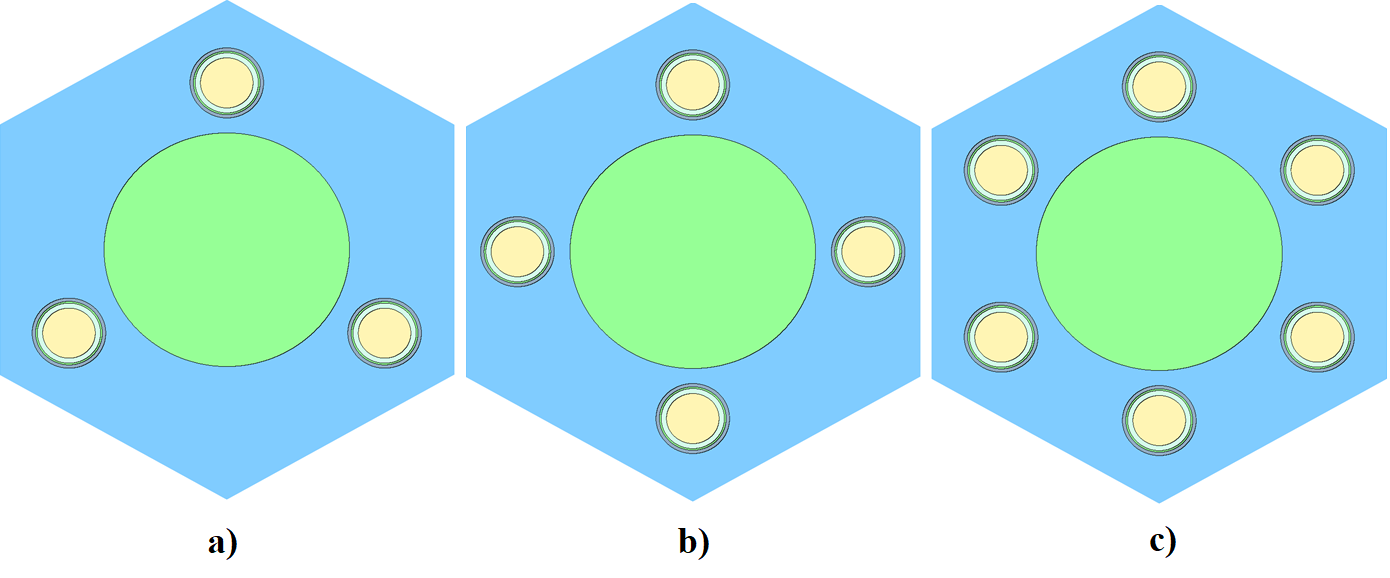
\includegraphics[width=\textwidth]{3_CR.png}
	\vspace{-0.5in}
	\caption{$XY$ section of graphite element with a) 3-CRs b) 4-CR c) 6-CRs configurations.} 
	\label{fig:3_CR}
\end{figure}

\begin{figure}[!ht]
	\centering
	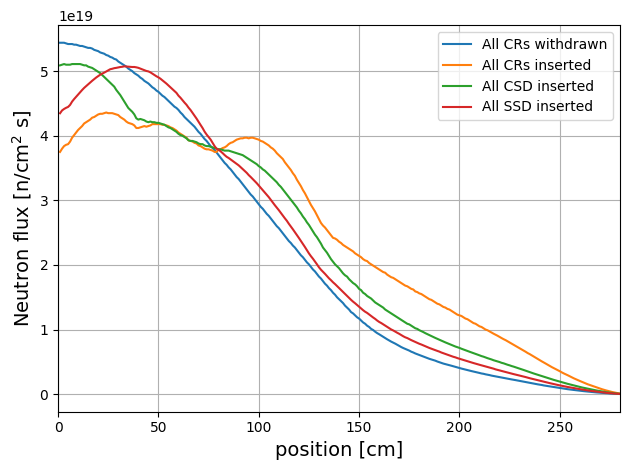
\includegraphics[width=\textwidth]{totalflux.png}
	\vspace{-0.5in}
	\caption{Radial neutron flux distribution at the mid-core for different 
	CR positions (CRs made of B$_4$C-90).} 
	\label{fig:totalflux}
\end{figure}
 

\subsubsection{Integral and differential CRW}

The integral CRWs are calculated for three different systems: all CRs, CSD, and SSD systems. We calculated the differential CRWs for the CSD system only because special adjusting rods (i.e., CSD) were assumed to adjust the reactivity.
The CRs are inserted gradually into the core from the top to the bottom. 
Equations~\ref{Equ:4} and~\ref{Equ:5} are used to calculate the integral and 
differential CRW, respectively. Figure~\ref{fig:integ} illustrates the integral CRW for CRs 
made of B$_4$C-90. The maximum integral worth of all CRs, CSD, and SSD 
clusters are about $14978$ $pcm$, $7914$ $pcm$, and $4998$ $pcm$, respectively. The 
integral worth of SSD clusters made of B$_4$C-90 is sufficient to shut down the reactor from any 
state.

The differential CRWs are demonstrated in Figure~\ref{fig:diff}. Theoretically, at the top of the core, the CR insertion has little effect since this region has low thermal neutron flux. Thus the differential CRW has the lowest values in this region. The effect of CR insertion increases gradually near the center of the core. At the center of the core (region with maximum thermal neutron flux), the differential CRW is the largest and changes slowly with rod insertion. From the center of the core to the bottom, the differential CRW values decrease (region with low thermal neutron flux). Figure~\ref{fig:diff} shows that the maximum differential CRW is shifted toward the bottom of the core and the curve is not exactly symmetrical. This is due to the asymmetrical distribution of the fuel and graphite in simulation \cite{xuemei2013study,son2016control}.

Figure~\ref{fig:CSD} shows the integral CRW for only Control Safety Devices (CSD) clusters with six 
different absorbing materials. The results show that all absorbing materials 
have almost the same integral rod worth in the upper half of the core 
($<250$ cm from the upper boundary of the core). Further insertion of the 
CRs demonstrates that the strongest absorber, B$_4$C-90 outperforms other materials.
Notably, all results are based on steady-state calculations. 

\begin{figure}
	\centering
	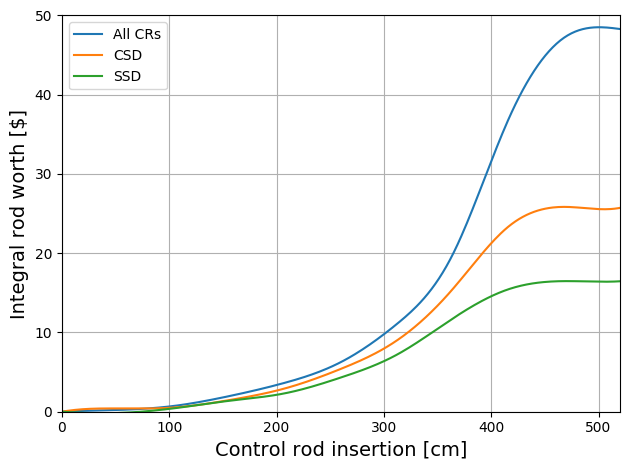
\includegraphics[width=\textwidth]{integ.png}
	\vspace{-0.5in}
	\caption{Integral CRW of all CRs, CSD, and SSD clusters (CRs made of B$_4$C-90).} 
	\label{fig:integ}
\end{figure}
\begin{figure}
	\centering
	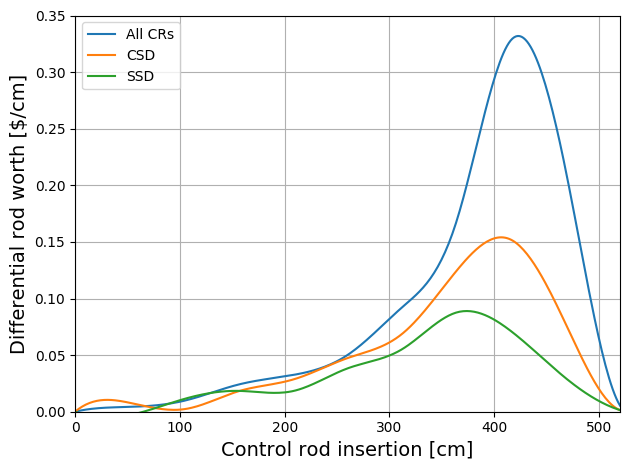
\includegraphics[width=\textwidth]{diff.png}
	\vspace{-0.5in}
	\caption{Differential CRW of CSD clusters (CRs made of B$_4$C-90).} 
	\label{fig:diff}
\end{figure}
\begin{figure}
	\centering
	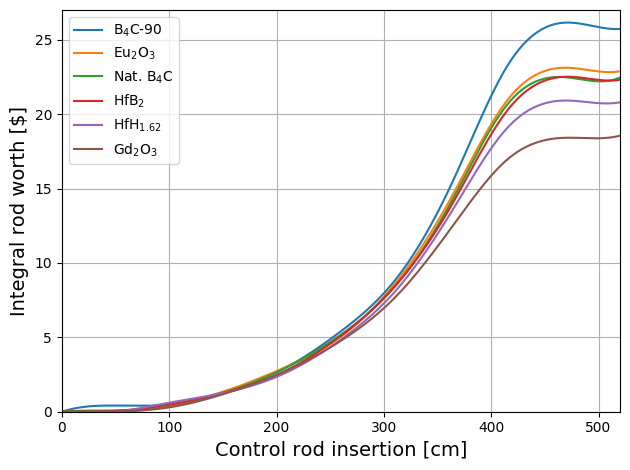
\includegraphics[width=\textwidth]{CSD.png}
	\vspace{-0.5in}
	\caption{Integral CRW of CSD clusters for various absorbing materials.} 
	\label{fig:CSD}
\end{figure}